\documentclass{fkpset}

% \newgeometry{bmargin=1in, tmargin=1.25in, lmargin=.75in, rmargin=.75in}
% \fancyhfoffset[R]{.05cm}

\name{Forest Kobayashi}
\class{Math 147}
\duedate{03/13/2019}
\assignment{HW 5 Solutions}

\chead{HW 5 Sample Solutions}
\rhead{Math 147 -- Spring, 2019}

\lfoot{Wednesday, March 13th 2019}

\problems{5.29, 5.32, 6.6, 6.11, 6.18}

\usepackage{hyperref}

\usetikzlibrary{hobby}

\newcommand{\tstd}{\ensuremath \ms T_{\rm std}}
\newcommand{\tprod}{\ensuremath \ms T_{\rm prod}}

\begin{document}
\pagestyle{plain}
\pagestyle{fancy}
  % \vspace{-2.9cm}
  \pointstable{}

  \vspace{1cm}

% --------------------------- Problem 1 ---------------------------- %
  \begin{problem}[5.29 (The Normality Lemma)]
    Let $A$ and $B$ be subsets of a topological space $X$ and let
    $\set{U_i}_{i \in \NN}$ and $\set{V_i}_{i \in \NN}$ be two
    collections of open sets such that
    \begin{enumerate}[label=(\arabic*)]
      \item $A \subset \bigcup_{i \in \NN} U_i$
      \item $B \subset \bigcup_{i \in \NN} V_i$
      \item For each $i \in \NN$, $\ol{U_i} \cap B = \varnothing$ and
        $\ol{V_i} \cap A = \varnothing$.
    \end{enumerate}
    Then there exist open sets $U$ and $V$ such that $A \subset U$, $B
    \subset V$, and $U \cap V = \varnothing$.
  \end{problem}
  \begin{leftbar}
    Before a solution, I'll give some intuition on how we might arrive
    at the candidate $U,V$ that work. Depict our two sets $A,B$ as
    follows:
    \begin{center}
      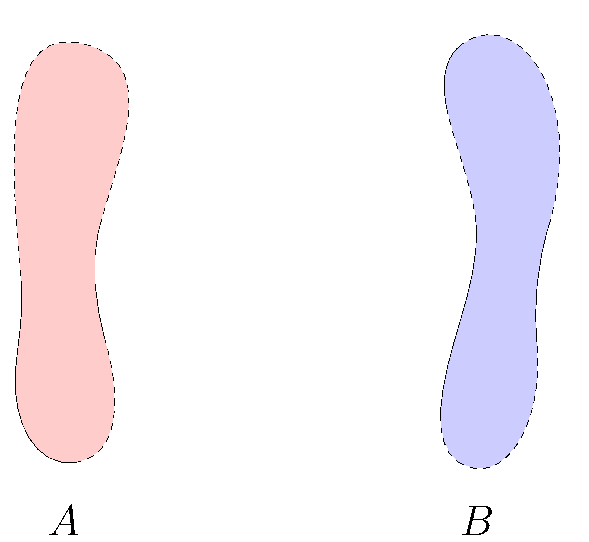
\includegraphics{figures/5-29-AB}
    \end{center}
    To make the TikZ easier, I'll draw our covers with boxes --- but
    note, in general they could be blobby. Anyways, we now draw
    $\ol{U_1}, \ol{V_1}$:
    \begin{center}
      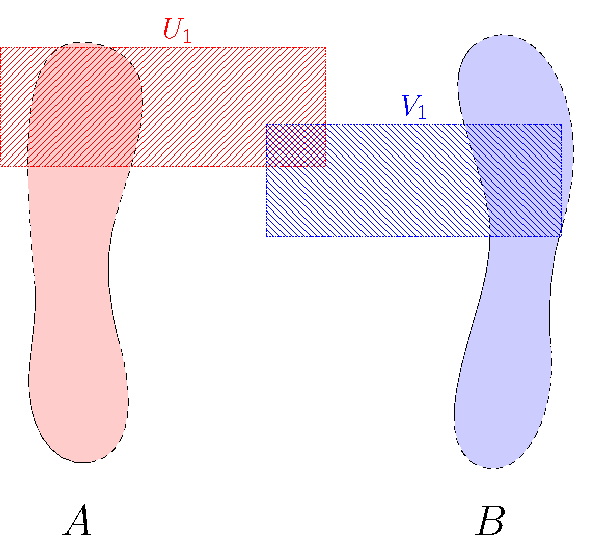
\includegraphics{figures/5-29-n=1}
    \end{center}
    We need to be sure that in our construction of $U$, we don't
    include any of the $V_i$. We want to use the $U_i$ somehow, but as
    we can see, they might intersect the $V_i$.
  \end{leftbar}
  \begin{solution}

  \end{solution}
  \clearpage

% --------------------------- Problem 2 ---------------------------- %

  \begin{problem}[5.32]
    Suppose a space $X$ is regular and has a countable basis. Then $X$
    is normal.
  \end{problem}
  \begin{solution}
    Let $A,B$ be disjoint closed sets.
  \end{solution}
  \clearpage

% --------------------------- Problem 3 ---------------------------- %
  \begin{problem}[6.6]
    The space $2^\RR$ is separable.
  \end{problem}
  \begin{solution}
  \end{solution}
  \clearpage

% --------------------------- Problem 4 ---------------------------- %
  \begin{problem}[6.11]
    Every uncountable set in a 2\textsuperscript{nd} countable space
    has a limit point.
  \end{problem}
  \begin{solution}
  \end{solution}
  \clearpage

% --------------------------- Problem 5 ---------------------------- %
  \begin{problem}[6.18]
    Suppose $x$ is a limit point of the set $A$ in a
    1\textsuperscript{st} countable space $X$. Then there is a
    sequence of points $\set{a_i}_{i \in \NN}$ that converges to $x$.
  \end{problem}
  \begin{solution}
  \end{solution}

\end{document}